\chapter{Estudio de viabilidad}

El desarrollo de cualquier proyecto tecnológico requiere un análisis exhaustivo de su viabilidad antes de su implementación. En este capítulo se presentan dos herramientas fundamentales para evaluar la factibilidad de SIDManager: el Lean Canvas, que proporciona una visión estratégica del proyecto, y un análisis de riesgos detallado que anticipa posibles desafíos y sus correspondientes planes de mitigación.

\section{Lean Canvas: Modelado ágil del proyecto}

El Lean Canvas de SIDManager (Figura \ref{fig:lean-canvas}) sintetiza los elementos clave del proyecto en nueve bloques estratégicos que analizamos detalladamente:

\begin{figure}
    \centering
    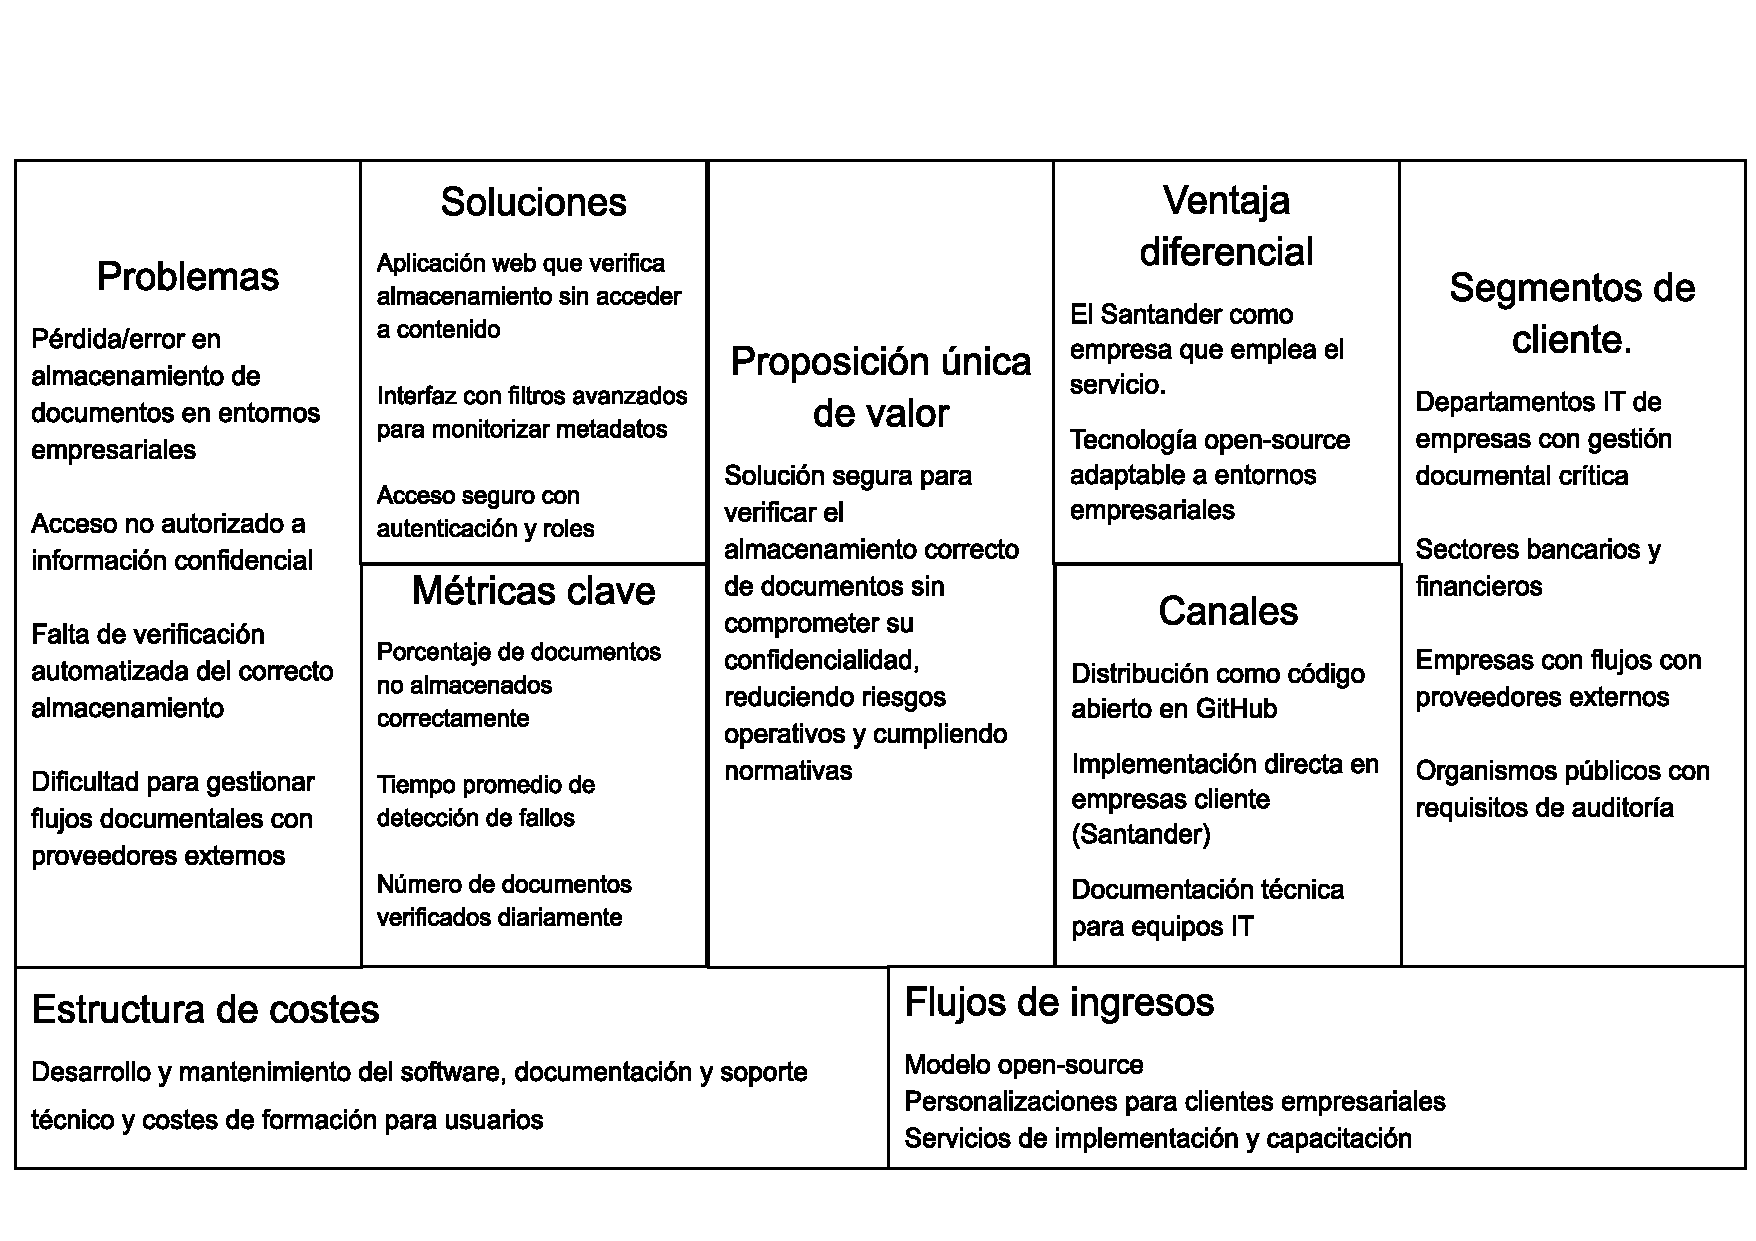
\includegraphics[width=1\linewidth]{imagenes/lean canvas tfg.pdf}
    \caption{Lean Canvas de SIDManager}
    \label{fig:lean-canvas}
\end{figure}

\subsection{Problemas identificados}
El canvas destaca cuatro problemáticas principales en la gestión documental empresarial:
\begin{itemize}
    \item Pérdidas y errores en el almacenamiento de documentos
    \item Riesgos de acceso no autorizado a información confidencial
    \item Falta de mecanismos automatizados para verificar el almacenamiento correcto
    \item Dificultades en la gestión de flujos documentales con proveedores externos
\end{itemize}

\subsection{Solución tecnológica}
La propuesta se articula en tres componentes fundamentales:
\begin{itemize}
    \item Aplicación web de verificación sin acceso a contenido confidencial
    \item Interfaz con sistema avanzado de filtrado de metadatos
    \item Arquitectura de seguridad con autenticación robusta y gestión de roles
\end{itemize}

\subsection{Métricas de éxito}
Se establecen tres indicadores clave de rendimiento (KPIs):
\begin{itemize}
    \item Tasa de documentos mal almacenados (\%)
    \item Tiempo medio de detección de anomalías
    \item Volumen diario de documentos verificados
\end{itemize}

\subsection{Propuesta de valor}
La singularidad de SIDManager radica en su capacidad para:
\begin{itemize}
    \item Garantizar la integridad documental sin comprometer la confidencialidad
    \item Reducir riesgos operativos en procesos críticos
    \item Cumplir con normativas de protección de datos (GDPR, etc.)
\end{itemize}

\subsection{Ventaja competitiva}
Dos factores diferenciadores:
\begin{itemize}
    \item Caso de uso real en entidad bancaria (Santander) como validación temprana
    \item Modelo open-source con adaptabilidad a entornos empresariales complejos
\end{itemize}

\subsection{Segmentación de clientes}
Los principales mercados objetivo incluyen:
\begin{itemize}
    \item Departamentos IT de empresas con gestión documental crítica
    \item Sector bancario y financiero (clientes primarios)
    \item Organismos públicos con exigentes requisitos de auditoría
    \item Empresas con flujos documentales externos complejos
\end{itemize}

\subsection{Modelo de distribución}
Estrategia multicanal:
\begin{itemize}
    \item Publicación como código abierto en GitHub
    \item Implementación directa en clientes corporativos
    \item Documentación técnica especializada para equipos IT
\end{itemize}

\subsection{Estructura económica}
\begin{itemize}
    \item Costes principales: Desarrollo de software, mantenimiento, soporte técnico y formación
    \item Flujos de ingresos: 
    \begin{itemize}
        \item Modelo open-source (versión base gratuita)
        \item Personalizaciones para clientes empresariales
        \item Servicios profesionales de implementación
    \end{itemize}
\end{itemize}

\section{Evaluación de riesgos}
Cada riesgo ha sido evaluado según dos parámetros fundamentales en la tabla \ref{table:risk-table}:
\begin{itemize}
    \item Probabilidad: Baja ( 0 - 30 \%), Moderada ( 30 - 70 \%), Alta ( 70 - 100 \%)
    \item Impacto: Tolerable (afecta plazos menores), Serio (compromete funcionalidades), Crítico (pone en peligro el proyecto)
\end{itemize}

\begin{table}
    \caption{Tabla de evaluación de riesgos}
    \label{table:risk-table}
    \begin{center}
    
    \begin{longtable}{|>{\raggedright\arraybackslash}p{3cm}|>{\raggedright\arraybackslash}p{3cm}|>{\raggedright\arraybackslash}p{2cm}|>{\raggedright\arraybackslash}p{6cm}|}
    \hline
    \textbf{Riesgo} & \textbf{Probabilidad} & \textbf{Efecto} & \textbf{Estrategia} \\
    \hline
    \endhead
    
    \hline
    \multicolumn{4}{|c|}{\textbf{Riesgos Tecnológicos}} \\
    \hline
    
    Desconocimiento al utilizar Spring Boot, JPA y Thymeleaf & Moderada & Tolerable & 
    \begin{itemize}
    \item Prevención: Realizar cursos y tutoriales sobre las tecnologías antes de comenzar el desarrollo
    \item Minimización: Consultar documentación oficial y ejemplos de proyectos similares
    \item Contingencia: Usar tecnologías alternativas más conocidas como Angular o React si fuera necesario
    \end{itemize} \\
    \hline
    
    Problemas de compatibilidad entre versiones de las tecnologías & Baja & Serio &
    \begin{itemize}
    \item Prevención: Verificar compatibilidad entre versiones antes de comenzar
    \item Minimización: Usar versiones LTS (Long Term Support) de las tecnologías
    \item Contingencia: Mantener versiones anteriores hasta resolver los conflictos
    \end{itemize} \\
    \hline
    
    Rendimiento insuficiente con grandes volúmenes de documentos & Moderada & Serio &
    \begin{itemize}
    \item Prevención: Diseñar consultas optimizadas y usar paginación
    \item Minimización: Implementar caché para consultas frecuentes
    \item Contingencia: Limitar el número de documentos mostrados por consulta
    \end{itemize} \\
    \hline
    
    \multicolumn{4}{|c|}{\textbf{Riesgos Personales}} \\
    \hline
    
    Falta de experiencia en desarrollo de aplicaciones empresariales & Alta & Tolerable &
    \begin{itemize}
    \item Prevención: Asignar tiempo extra para investigación y aprendizaje
    \item Minimización: Consultar con tutores y compañeros con más experiencia
    \item Contingencia: Simplificar funcionalidades complejas en primera iteración
    \end{itemize} \\
    \hline
    
    Problemas de gestión del tiempo & Moderada & Serio &
    \begin{itemize}
    \item Prevención: Crear un cronograma detallado con hitos claros
    \item Minimización: Usar metodologías ágiles con sprints cortos
    \item Contingencia: Priorizar funcionalidades esenciales para MVP
    \end{itemize} \\
    \hline
    
    \multicolumn{4}{|c|}{\textbf{Riesgos de Organización}} \\
    \hline
    
    Cambios en los requerimientos durante el desarrollo & Moderada & Serio &
    \begin{itemize}
    \item Prevención: Documentar exhaustivamente los requerimientos iniciales
    \item Minimización: Mantener comunicación constante con los stakeholders
    \item Contingencia: Usar diseño modular para facilitar cambios
    \end{itemize} \\
    \hline
    
    Dependencia de terceros (empresa colaboradora) & Baja & Crítico &
    \begin{itemize}
    \item Prevención: Establecer acuerdos claros desde el inicio
    \item Minimización: Mantener comunicación periódica
    \item Contingencia: Desarrollar versión simulada de los servicios externos
    \end{itemize} \\
    \hline
    
    \multicolumn{4}{|c|}{\textbf{Riesgos de Herramientas}} \\
    \hline
    
    Problemas con la configuración de Spring Security & Moderada & Serio &
    \begin{itemize}
    \item Prevención: Estudiar a fondo la documentación de Spring Security
    \item Minimización: Implementar configuración por pasos con pruebas intermedias
    \item Contingencia: Usar soluciones de autenticación más simples inicialmente
    \end{itemize} \\
    \hline
    
    Dificultades con la integración de Thymeleaf & Baja & Tolerable &
    \begin{itemize}
    \item Prevención: Realizar prototipos iniciales con Thymeleaf
    \item Minimización: Usar fragmentos reutilizables y layouts
    \item Contingencia: Considerar el uso de herramientas alternativas
    \end{itemize} \\
    \hline
    
    \multicolumn{4}{|c|}{\textbf{Riesgos de Requerimientos}} \\
    \hline
    
    Requerimientos de seguridad demasiado exigentes & Alta & Serio &
    \begin{itemize}
    \item Prevención: Analizar minuciosamente los requerimientos de seguridad
    \item Minimización: Implementar Spring Security desde el inicio del proyecto
    \item Contingencia: Priorizar las medidas de seguridad más críticas
    \end{itemize} \\
    \hline
    
    Dificultad en la validación de documentos sin acceder a metadatos & Moderada & Serio &
    \begin{itemize}
    \item Prevención: Estudiar alternativas técnicas para la validación
    \item Minimización: Consultar con expertos en seguridad de datos
    \item Contingencia: Proponer un método alternativo de verificación
    \end{itemize} \\
    \hline
    
    \multicolumn{4}{|c|}{\textbf{Otros Riesgos}} \\
    \hline
    
    Problemas con la base de datos en producción & Baja & Crítico &
    \begin{itemize}
    \item Prevención: Realizar copias de seguridad periódicas
    \item Minimización: Implementar scripts de migración y recuperación
    \item Contingencia: Tener un entorno de desarrollo independiente
    \end{itemize} \\
    \hline
    
    \end{longtable}
    \end{center}
\end{table}

\section{Conclusiones de viabilidad}
El análisis conjunto del Lean Canvas y la matriz de riesgos permite concluir que:
\begin{enumerate}
    \item El proyecto es técnicamente viable, aunque requiere inversión inicial en capacitación.
    \item La viabilidad económica está garantizada por el modelo de ingresos escalable.
    \item Los riesgos identificados son gestionables mediante las estrategias propuestas.
    \item El factor crítico de éxito reside en el equilibrio entre seguridad y usabilidad.
\end{enumerate}

Por tanto, el estudio demuestra que SIDManager aborda una necesidad real del mercado con una solución técnicamente robusta, posicionándose como una alternativa viable frente a soluciones existentes como Alfresco o OpenKM. Los siguientes capítulos detallarán la implementación concreta de las estrategias aquí esbozadas.